\tikzset{every picture/.style={line width=0.75pt}} %set default line width to 0.75pt        

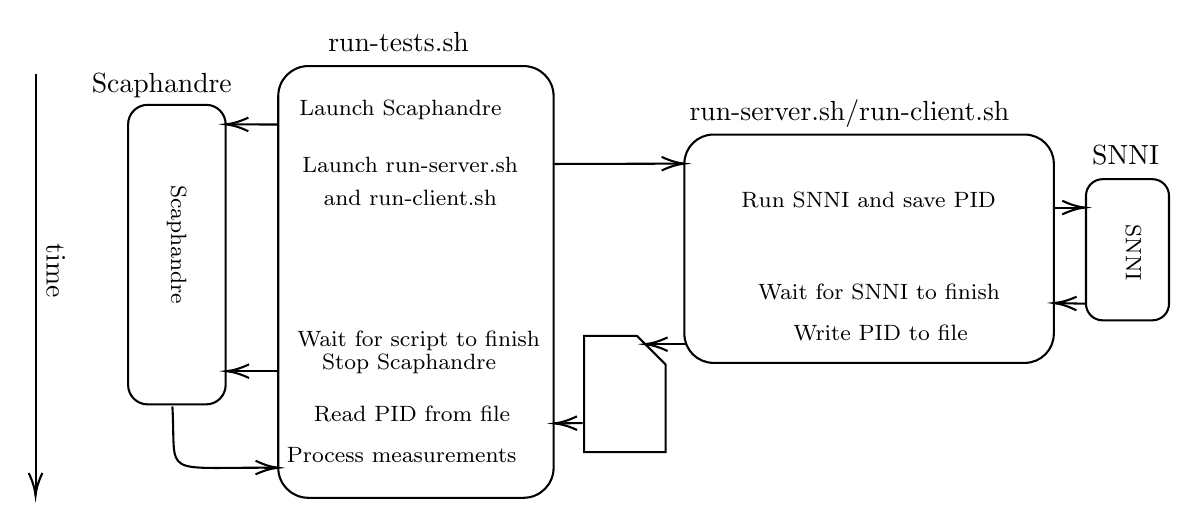
\begin{tikzpicture}[x=0.75pt,y=0.75pt,yscale=-1,xscale=1]
%uncomment if require: \path (0,300); %set diagram left start at 0, and has height of 300

%Rounded Rect [id:dp030762214985281755] 
\draw   (163.33,82.46) .. controls (163.33,74.47) and (169.81,68) .. (177.79,68) -- (281.54,68) .. controls (289.53,68) and (296,74.47) .. (296,82.46) -- (296,261.54) .. controls (296,269.53) and (289.53,276) .. (281.54,276) -- (177.79,276) .. controls (169.81,276) and (163.33,269.53) .. (163.33,261.54) -- cycle ;
%Rounded Rect [id:dp40135169613462107] 
\draw   (359,115) .. controls (359,107.27) and (365.27,101) .. (373,101) -- (523,101) .. controls (530.73,101) and (537,107.27) .. (537,115) -- (537,197) .. controls (537,204.73) and (530.73,211) .. (523,211) -- (373,211) .. controls (365.27,211) and (359,204.73) .. (359,197) -- cycle ;
%Rounded Rect [id:dp2296582029018056] 
\draw   (552.5,130.5) .. controls (552.5,126.08) and (556.08,122.5) .. (560.5,122.5) -- (584.5,122.5) .. controls (588.92,122.5) and (592.5,126.08) .. (592.5,130.5) -- (592.5,182.5) .. controls (592.5,186.92) and (588.92,190.5) .. (584.5,190.5) -- (560.5,190.5) .. controls (556.08,190.5) and (552.5,186.92) .. (552.5,182.5) -- cycle ;
%Straight Lines [id:da8751872721660255] 
\draw    (296.33,115.17) -- (357,115.01) ;
\draw [shift={(359,115)}, rotate = 179.85] [color={rgb, 255:red, 0; green, 0; blue, 0 }  ][line width=0.75]    (10.93,-3.29) .. controls (6.95,-1.4) and (3.31,-0.3) .. (0,0) .. controls (3.31,0.3) and (6.95,1.4) .. (10.93,3.29)   ;
%Straight Lines [id:da5745846675961594] 
\draw    (537,136.17) -- (550,136.17) ;
\draw [shift={(552,136.17)}, rotate = 180] [color={rgb, 255:red, 0; green, 0; blue, 0 }  ][line width=0.75]    (10.93,-3.29) .. controls (6.95,-1.4) and (3.31,-0.3) .. (0,0) .. controls (3.31,0.3) and (6.95,1.4) .. (10.93,3.29)   ;
%Straight Lines [id:da22191721271792242] 
\draw    (552.5,182.5) -- (539,182.21) ;
\draw [shift={(537,182.17)}, rotate = 1.23] [color={rgb, 255:red, 0; green, 0; blue, 0 }  ][line width=0.75]    (10.93,-3.29) .. controls (6.95,-1.4) and (3.31,-0.3) .. (0,0) .. controls (3.31,0.3) and (6.95,1.4) .. (10.93,3.29)   ;
%Snip Single Corner Rect [id:dp8679720350977688] 
\draw   (310.67,198) -- (336.23,198) -- (350,211.77) -- (350,254) -- (310.67,254) -- cycle ;
%Straight Lines [id:da7502278744460461] 
\draw    (360,202) -- (342,202) ;
\draw [shift={(340,202)}, rotate = 360] [color={rgb, 255:red, 0; green, 0; blue, 0 }  ][line width=0.75]    (10.93,-3.29) .. controls (6.95,-1.4) and (3.31,-0.3) .. (0,0) .. controls (3.31,0.3) and (6.95,1.4) .. (10.93,3.29)   ;
%Straight Lines [id:da6953182839576503] 
\draw    (310,240) -- (298.33,240.14) ;
\draw [shift={(296.33,240.17)}, rotate = 359.3] [color={rgb, 255:red, 0; green, 0; blue, 0 }  ][line width=0.75]    (10.93,-3.29) .. controls (6.95,-1.4) and (3.31,-0.3) .. (0,0) .. controls (3.31,0.3) and (6.95,1.4) .. (10.93,3.29)   ;
%Rounded Rect [id:dp8590315960302918] 
\draw   (91,96.07) .. controls (91,90.88) and (95.21,86.67) .. (100.4,86.67) -- (128.6,86.67) .. controls (133.79,86.67) and (138,90.88) .. (138,96.07) -- (138,221.6) .. controls (138,226.79) and (133.79,231) .. (128.6,231) -- (100.4,231) .. controls (95.21,231) and (91,226.79) .. (91,221.6) -- cycle ;
%Straight Lines [id:da37936349291138083] 
\draw    (163,96.17) -- (140,96.07) ;
\draw [shift={(138,96.07)}, rotate = 0.23] [color={rgb, 255:red, 0; green, 0; blue, 0 }  ][line width=0.75]    (10.93,-3.29) .. controls (6.95,-1.4) and (3.31,-0.3) .. (0,0) .. controls (3.31,0.3) and (6.95,1.4) .. (10.93,3.29)   ;
%Straight Lines [id:da9099882740378028] 
\draw    (163.33,215) -- (140.33,215) ;
\draw [shift={(138.33,215)}, rotate = 360] [color={rgb, 255:red, 0; green, 0; blue, 0 }  ][line width=0.75]    (10.93,-3.29) .. controls (6.95,-1.4) and (3.31,-0.3) .. (0,0) .. controls (3.31,0.3) and (6.95,1.4) .. (10.93,3.29)   ;
%Curve Lines [id:da6242806346709759] 
\draw    (112.33,232) .. controls (114.31,266.65) and (105.51,261.12) .. (161.61,261.53) ;
\draw [shift={(163.33,261.54)}, rotate = 180.54] [color={rgb, 255:red, 0; green, 0; blue, 0 }  ][line width=0.75]    (10.93,-3.29) .. controls (6.95,-1.4) and (3.31,-0.3) .. (0,0) .. controls (3.31,0.3) and (6.95,1.4) .. (10.93,3.29)   ;
%Straight Lines [id:da4194250785386484] 
\draw    (46.4,71.8) -- (46.4,273) ;
\draw [shift={(46.4,275)}, rotate = 270] [color={rgb, 255:red, 0; green, 0; blue, 0 }  ][line width=0.75]    (10.93,-3.29) .. controls (6.95,-1.4) and (3.31,-0.3) .. (0,0) .. controls (3.31,0.3) and (6.95,1.4) .. (10.93,3.29)   ;

% Text Node
\draw (172,83) node [anchor=north west][inner sep=0.75pt]   [align=left] {{\footnotesize Launch Scaphandre}};
% Text Node
\draw (171,110.4) node [anchor=north west][inner sep=0.75pt]   [align=left] {\begin{minipage}[lt]{81.6pt}\setlength\topsep{0pt}
\begin{center}
{\footnotesize Launch run-server.sh }\\{\footnotesize and run-client.sh}
\end{center}

\end{minipage}};
% Text Node
\draw (385,127.4) node [anchor=north west][inner sep=0.75pt]   [align=left] {{\footnotesize Run SNNI and save PID}};
% Text Node
\draw (186,50) node [anchor=north west][inner sep=0.75pt]   [align=left] {run-tests.sh};
% Text Node
\draw (360,82.5) node [anchor=north west][inner sep=0.75pt]   [align=left] {run-server.sh/run-client.sh};
% Text Node
\draw (554,105) node [anchor=north west][inner sep=0.75pt]   [align=left] {SNNI};
% Text Node
\draw (393,171.4) node [anchor=north west][inner sep=0.75pt]   [align=left] {{\footnotesize Wait for SNNI to finish}};
% Text Node
\draw (410,191.4) node [anchor=north west][inner sep=0.75pt]   [align=left] {{\footnotesize Write PID to file}};
% Text Node
\draw (580.5,142.9) node [anchor=north west][inner sep=0.75pt]  [rotate=-90] [align=left] {{\footnotesize SNNI}};
% Text Node
\draw (171,194.4) node [anchor=north west][inner sep=0.75pt]   [align=left] {{\footnotesize Wait for script to finish}};
% Text Node
\draw (179,230.4) node [anchor=north west][inner sep=0.75pt]   [align=left] {{\footnotesize Read PID from file}};
% Text Node
\draw (183,205.4) node [anchor=north west][inner sep=0.75pt]   [align=left] {{\footnotesize Stop Scaphandre}};
% Text Node
\draw (166,250.4) node [anchor=north west][inner sep=0.75pt]   [align=left] {{\footnotesize Process measurements}};
% Text Node
\draw (72,70) node [anchor=north west][inner sep=0.75pt]   [align=left] {Scaphandre};
% Text Node
\draw (120.62,123.83) node [anchor=north west][inner sep=0.75pt]  [rotate=-90] [align=left] {{\footnotesize Scaphandre}};
% Text Node
\draw (62.1,152.03) node [anchor=north west][inner sep=0.75pt]  [rotate=-90] [align=left] {time};


\end{tikzpicture}
